\subsection{The Standard Model of particle physics}

\begin{frame}{The Standard Model (SM) of particle physics}

\begin{columns}
\column{0.5\textwidth}

\begin{itemize}
    \item Quantum field theory, based on the principal gauge invariance $\textcolor{HHturquoise_d}{SU(3)}\times \textcolor{HHturquoise_l}{SU(2)}\times \textcolor{HHturquoise_l}{U(1)}$
    \item Unified \textcolor{HHturquoise_d}{Strong} and \textcolor{HHturquoise_l}{Electroweak} interactions.
    \item Fermions: matter particles
    \begin{itemize}
        \item \textcolor{violet}{Quarks}
        \item \textcolor{applegreen}{Leptons}
    \end{itemize}
    \item \textcolor{cadmiumorange}{Gauge bosons}: mediators of interactions
\end{itemize}    
\begin{itemize}    
    \item \textcolor{HHyellow}{Higgs boson}
    \begin{itemize}
        \item Scalar boson 
        \item Responsible for mass generation through EWSB mechanism
    \end{itemize}
\end{itemize}

\column{0.5\textwidth}
\begin{figure}
    \centering
    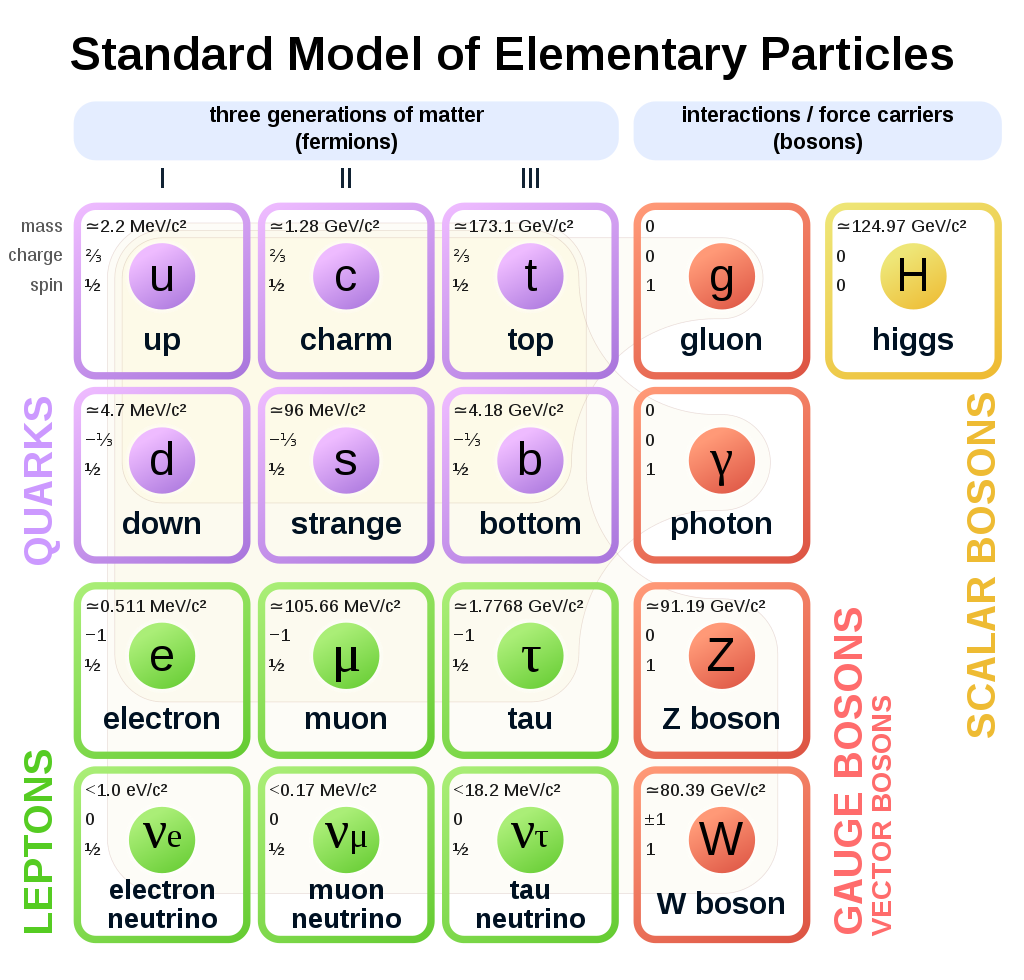
\includegraphics[width=1\textwidth]{Part1/Img/SM_particles.png}
\end{figure}
\end{columns}
\end{frame}

\begin{frame}{Electroweak Symmetry Breaking and Higgs boson}

\begin{columns}
\column{0.4\textwidth}
\begin{figure}
    \centering
    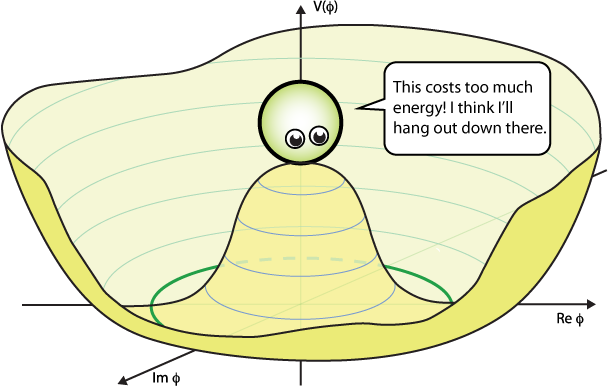
\includegraphics[width=0.8\textwidth]{Part1/Img/Higgs-Potential-lookdown.png}
\end{figure}
\begin{figure}
    \centering
    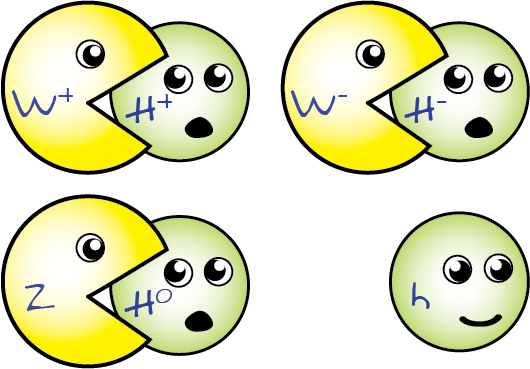
\includegraphics[width=0.8\textwidth]{Part1/Img/Goldstone-Eaten-four.png}
\end{figure}

\column{0.6\textwidth}
Hardcode of gauge boson mass terms break gauge symmetry of SM:
\begin{itemize}
    \item \textcolor{structurColor}{Brout-Englert-Higgs} include complex scalar field: $V(\phi^\dagger\phi) = \mu^2\phi^\dagger\phi + \lambda(\phi^\dagger\phi)^2$
    \item Choice of the vacuum state \textcolor{applegreen}{spontaneously breaks the symmetry}:
    \begin{itemize}
        \item Gauge bosons become massive
        \item Higgs boson arises: unknown mass
        \item Fermion masses: generated through Yukawa couplings
    \end{itemize}
\end{itemize}

\begin{itemize}
    \item \underline{Observed} in 2012 at LHC with a mass $m_{H} = $ 125 GeV
    \item \underline{Now}, most of Higgs parameters are measured: mass, cross-section, and coupling to fermions/bosons
    \item \textcolor{HHred}{Not all, Higgs boson self-coupling still resists to physicists}
\end{itemize}
\end{columns}
\end{frame}

\subsection{Higgs boson self-coupling}

\begin{frame}{Higgs boson self-coupling}
\begin{columns}
\column{0.6\textwidth}    
\begin{itemize}
    \item \textcolor{structurColor}{Higgs boson trilinear coupling} (self-coupling)
    \item controls the shape of the Higgs potential:
    \begin{itemize}
        \item Importance to experimentally reconstruct Higgs potential shape
    \end{itemize} 
    \item At SM, $\lambda^{SM} \sim 0.13$
    \item Deviations from SM, quantified as \textbf{\textcolor{HHred}{$\kappa_{\lambda} = \frac{\lambda}{\lambda^{SM}}$}}, may indicate new physics beyond SM (BSM)
    \item Only \underline{\textbf{direct}} access to measure it at the LHC, is through the \textcolor{HHturquoise_d}{Higgs boson pair (\textbf{HH}) production} (not observed yet).
\end{itemize}

\column{0.4\textwidth}    
\begin{equation*}
    V \supset \lambda v^2H^2 + \textcolor{HHred}{\lambda vH^3} + \frac{\lambda}{v}H^4
\end{equation*}

\begin{figure}
    \centering
    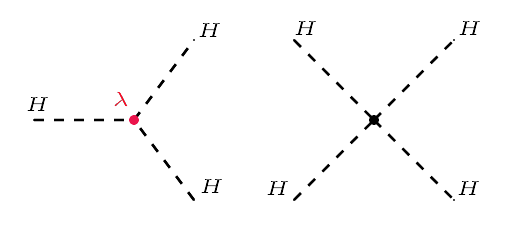
\includegraphics[width=0.9\textwidth]{Part1/Img/hhh_diagrams.png}
\end{figure}
\begin{equation*}
    \lambda = \frac{m_{H}^2}{2v^2}
\end{equation*}

\end{columns}    

\end{frame}

\subsection{Higgs boson pair production}

\begin{frame}{Higgs boson pair production at the LHC}

\begin{itemize}
    \item At the LHC, mainly produced via \underline{non-resonant} \textbf{\textcolor{HHred}{ggF}} and \textbf{\textcolor{HHturquoise_d}{VBF}} modes. 
\end{itemize}

\begin{figure}
    \fcolorbox{HHred}{HHwhite2}{     \subfloat{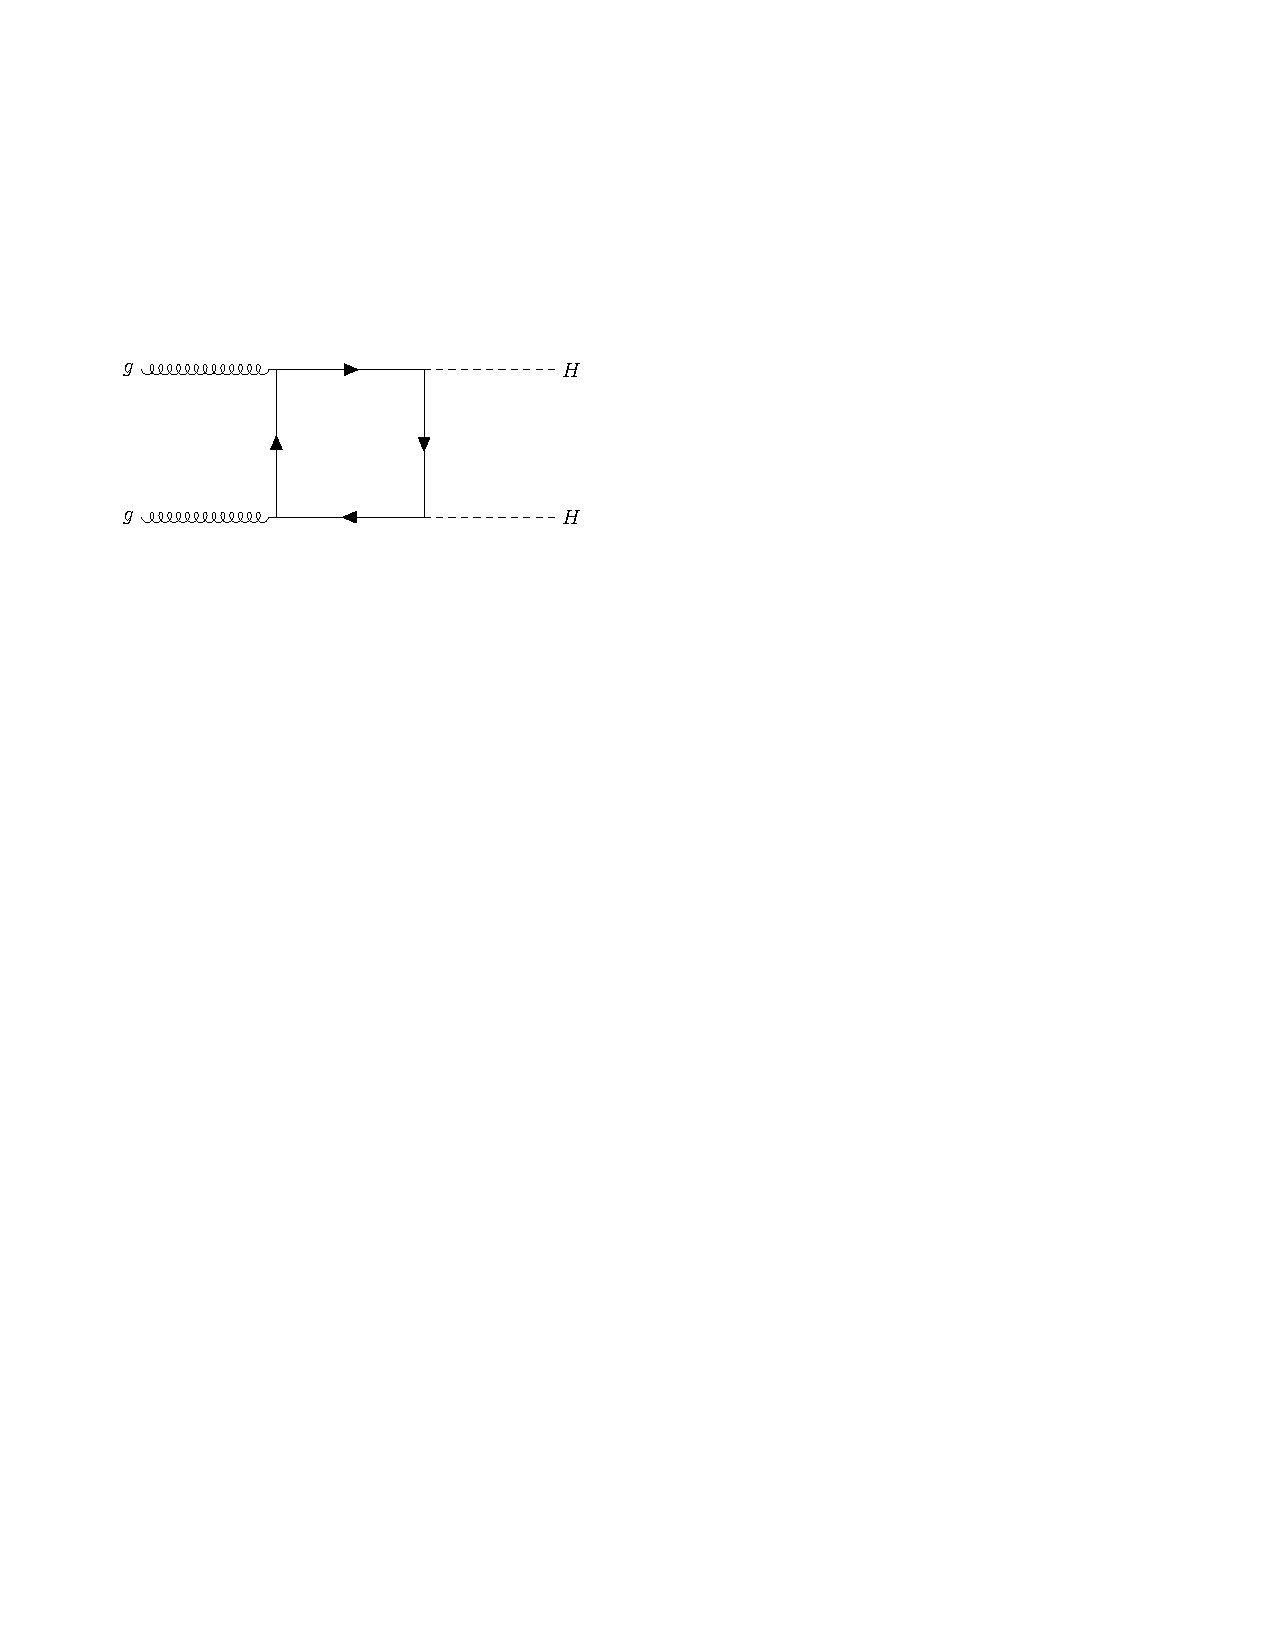
\includegraphics[width=0.25\textwidth]{Part1/Img/ggF_box.pdf}}
    \subfloat{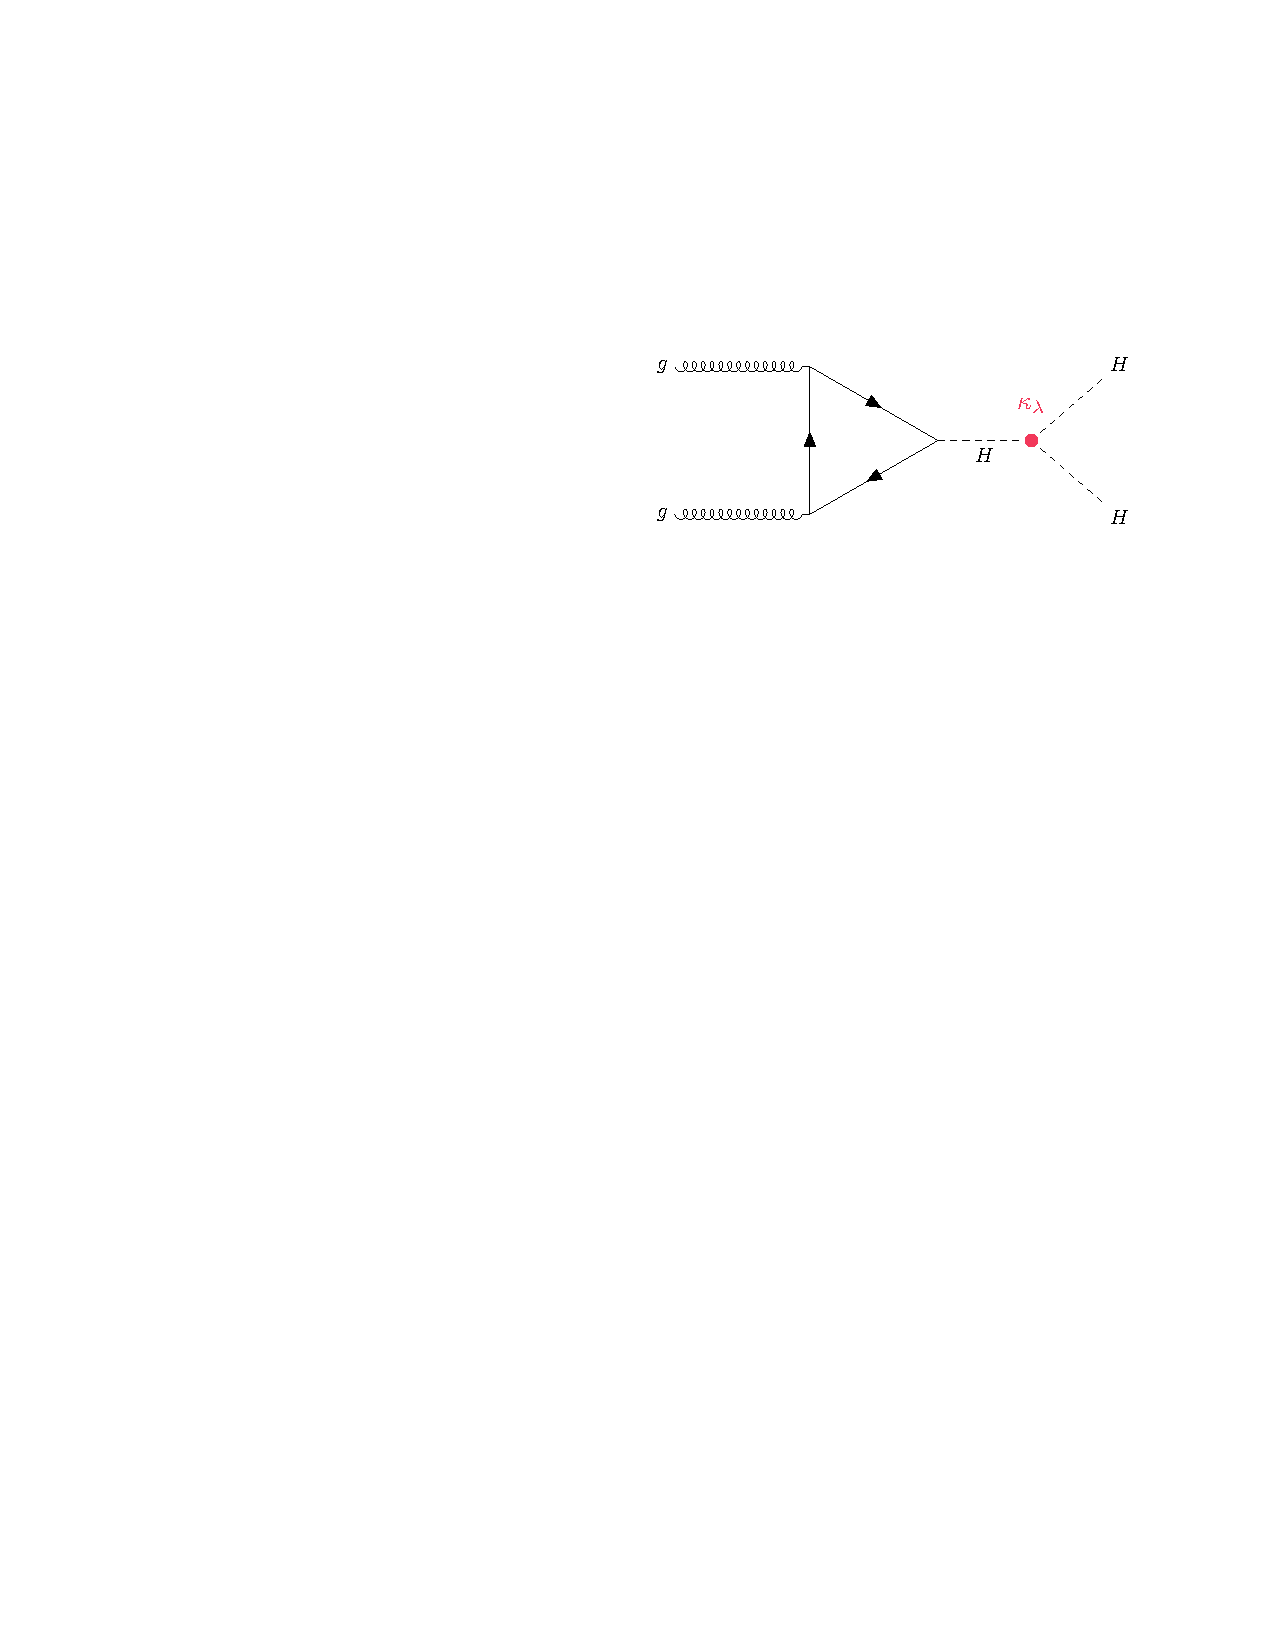
\includegraphics[width=0.25\textwidth]{Part1/Img/ggF_tri.pdf}}}
    \fcolorbox{HHturquoise_d}{HHwhite2}{
    \subfloat{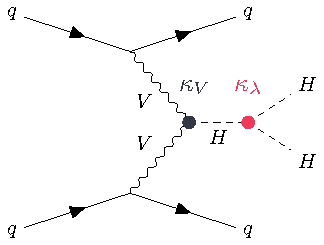
\includegraphics[width=0.17\textwidth]{Part1/Img/VBF_kvkl.pdf}}
    }
\end{figure}

\begin{columns}
\column{0.5\textwidth}  
\begin{figure}
    \centering
    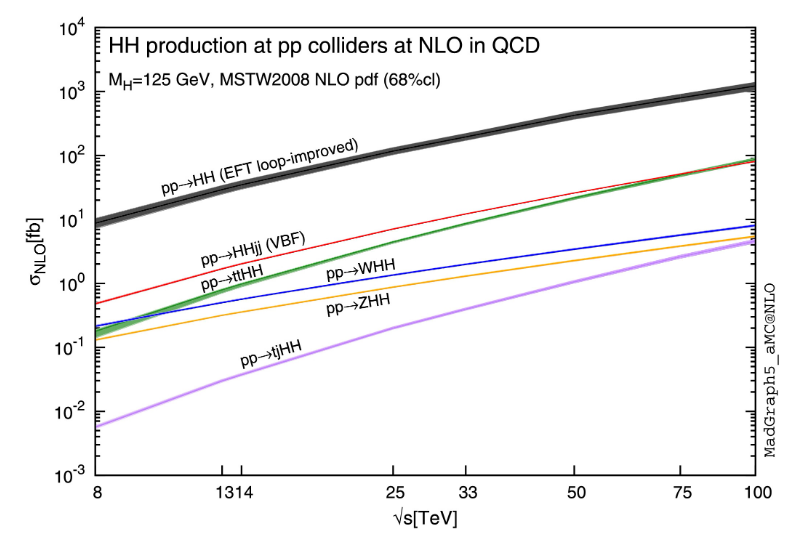
\includegraphics[width=0.8\textwidth]{Part1/Img/HH_XSec_as_S.png}
\end{figure}

\column{0.5\textwidth}  

\begin{itemize}
    \item At 13 TeV: 
    \begin{itemize}
        \item $\sigma^{ggF}_{HH} = $ 31.05 fb, 1000$\times$ smaller than $\sigma_{H}$
        \item $\sigma^{VBF}_{HH} = $ 1.73 fb, one order of magnitude smaller than ggF
    \end{itemize}
    \item HH can be reconstructed in different decay channels
\end{itemize}
\end{columns}
\end{frame}

\begin{frame}{Di-Higgs boson decay modes}

\begin{itemize}
    \item Combination of the decay modes of the two Higgs bosons
\end{itemize}
\begin{figure}
    \centering
    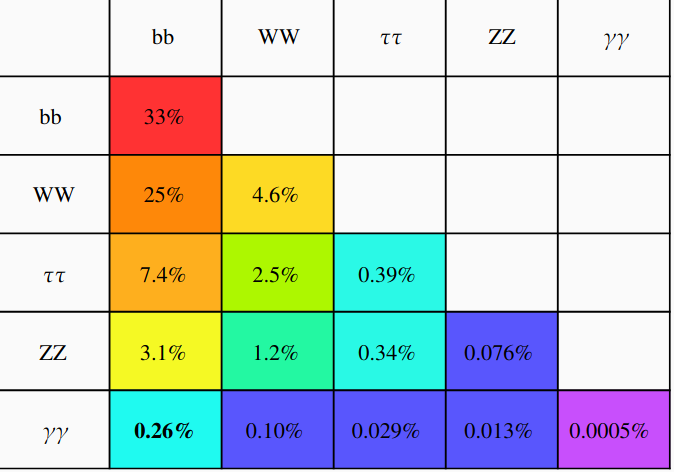
\includegraphics[width=0.45\textwidth]{Part1/Img/HH_decays.png}
\end{figure}
\begin{itemize}
    \item \textcolor{HHred}{Focusing on HH$\to b\bar{b}\gamma\gamma$}
    \item Despite low decay rate, one of the most sensitive channel:
    \begin{itemize}
        \item \textbf{High} H$\to b\bar{b}$ branching ratio
        \item Very \textbf{clean} signature
        \item \textbf{Excellent} $m_{\gamma\gamma}$ mass resolution
        \item \textbf{Good signal extraction}
    \end{itemize}
\end{itemize}

\end{frame}

\begin{frame}{Di-Higgs boson as a probe of BSM physics}

\begin{columns}
\column{0.6\textwidth} 
\begin{itemize}
    \item BSM physics can manifest as deviation:
    \begin{itemize}
        \item \textbf{\textcolor{HHred}{Total}} cross-section
        \item \textbf{\textcolor{HHturquoise_m}{Differential}} cross-section
    \end{itemize}
    \item Cross-section and kinematics depend on $\kappa_{\lambda}$ 
\end{itemize}
\underline{Thesis aim}: \textbf{search of HH events in the $b \bar{b}\gamma\gamma$ final state and constrain $\kappa_{\lambda}$}

\column{0.4\textwidth}  

\begin{figure}
    \centering
    \fcolorbox{HHred}{HHwhite2}{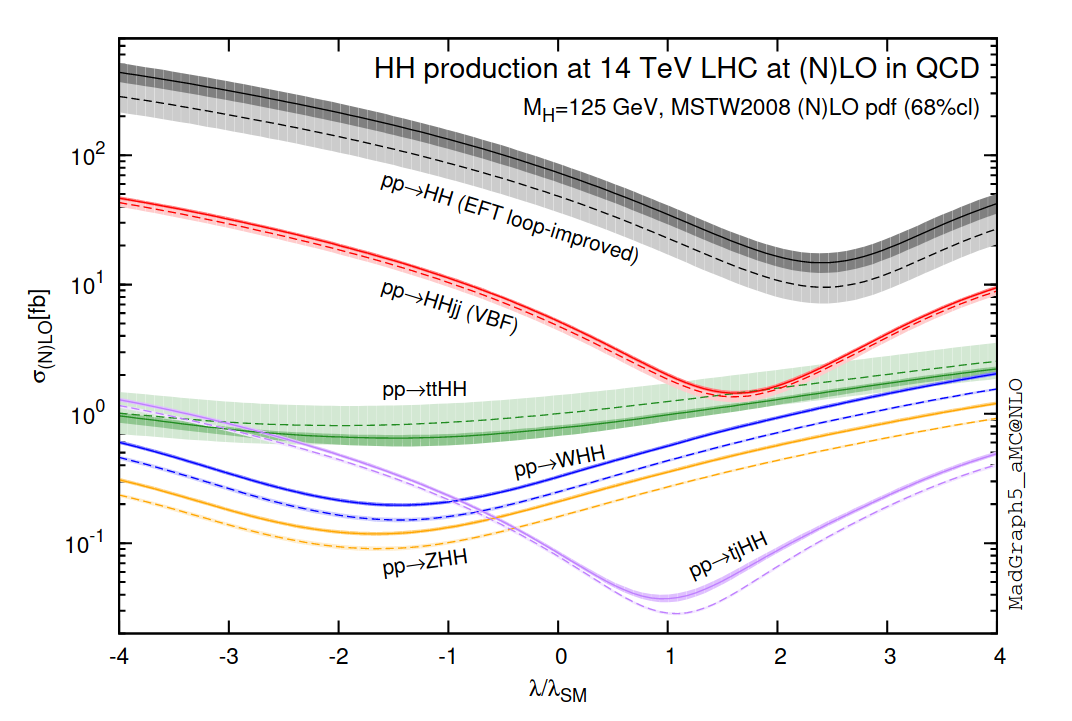
\includegraphics[width=0.7\textwidth]{Part1/Img/HH_Xsec_as_lambda.png}}
\end{figure}

\begin{figure}
    \centering
    \fcolorbox{HHturquoise_m}{HHwhite2}{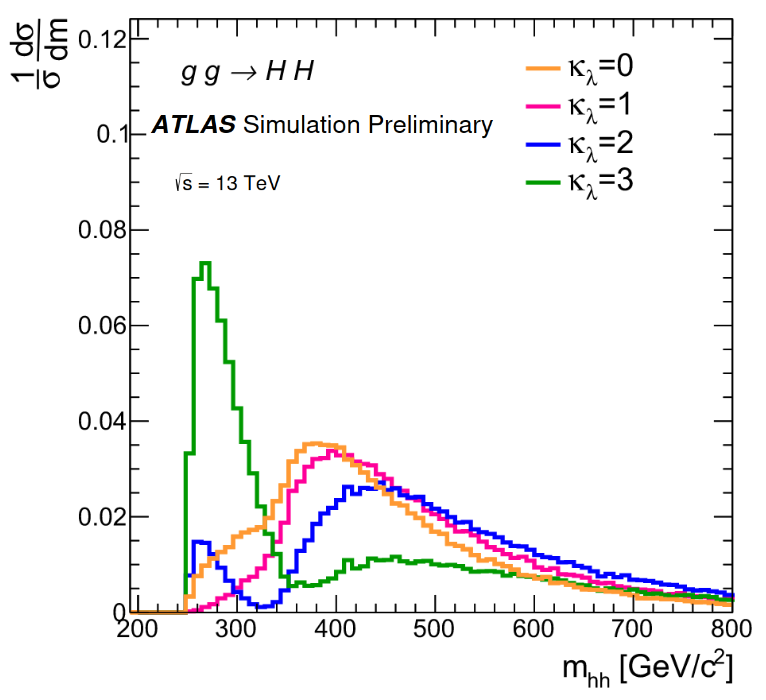
\includegraphics[width=0.7\textwidth]{Part1/Img/mHH.png}}
\end{figure}

\end{columns}



\end{frame}